\begin{figure}[t!]

  \setlength{\unitlength}{\textwidth}

  \begin{picture}(1,0.35)(0,0.725)

    \put(-0.01,0.76){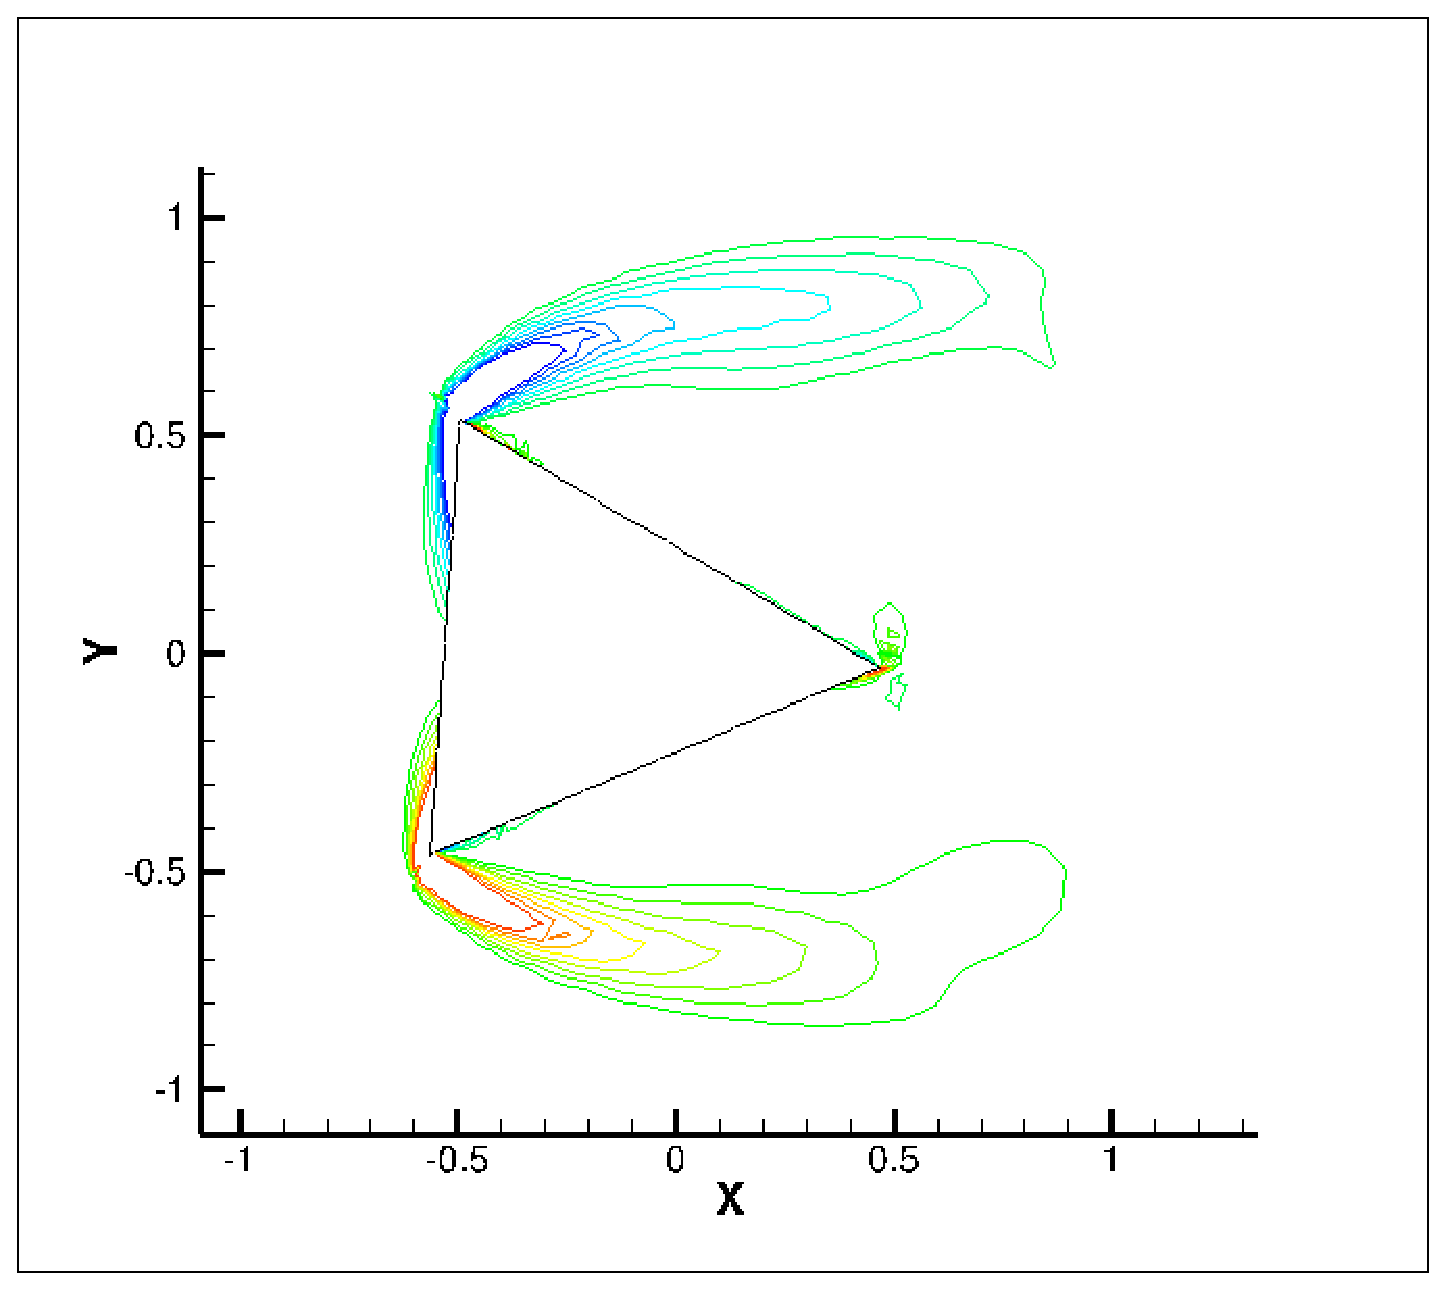
\includegraphics[width=0.33\unitlength]{./chapter-cross-sections/fnp/4.eps}}
    \put(0.335,0.76){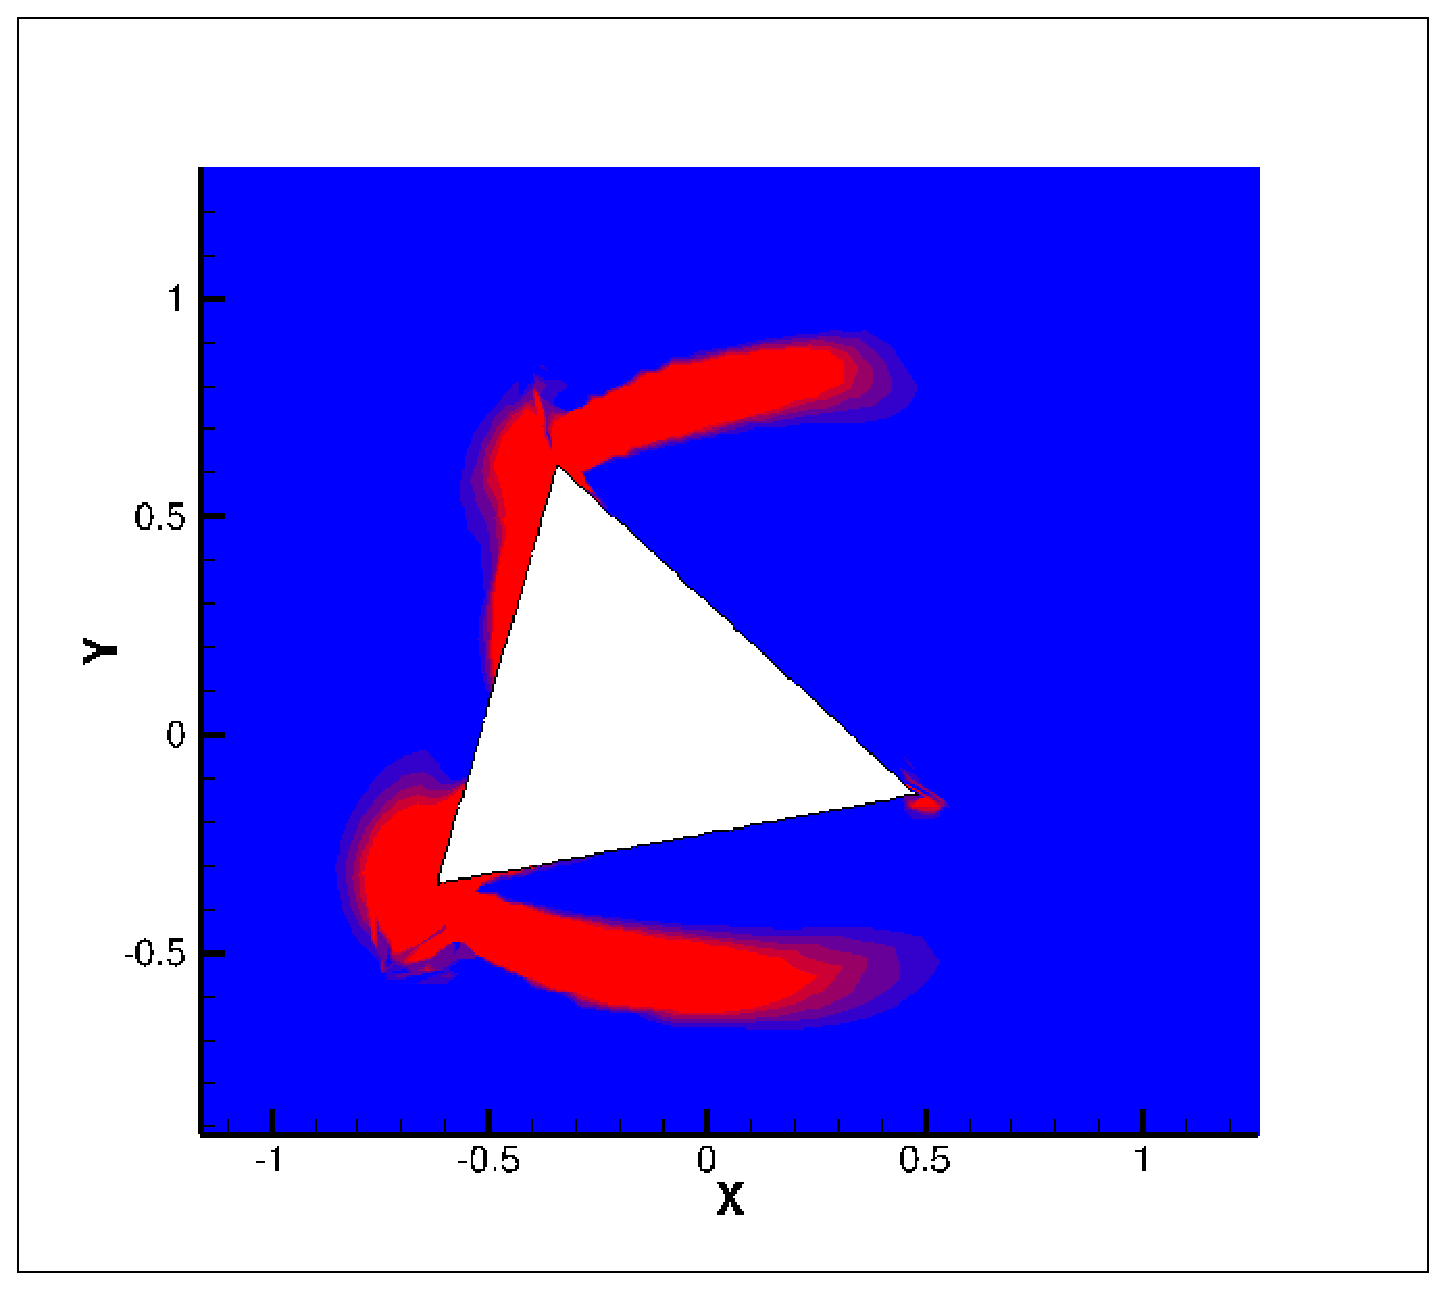
\includegraphics[width=0.33\unitlength]{./chapter-cross-sections/fnp/16.eps}}
    \put(0.68,0.76){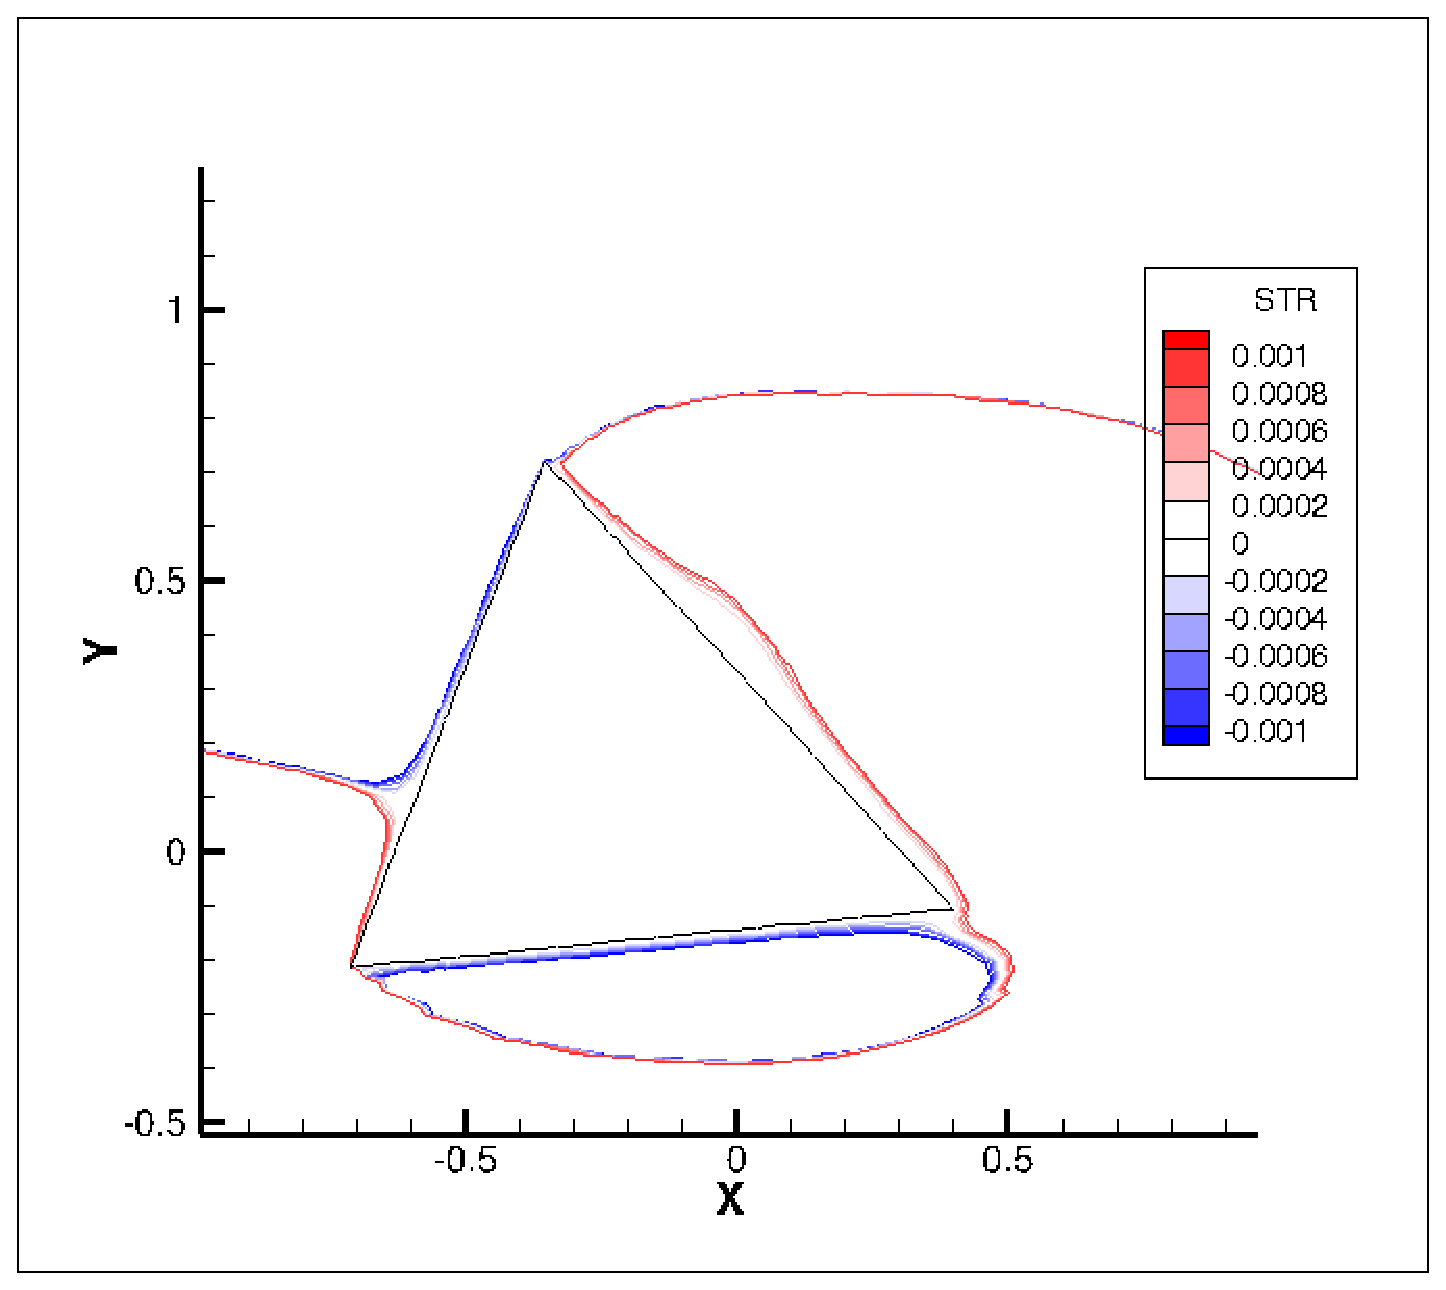
\includegraphics[width=0.33\unitlength]{./chapter-cross-sections/fnp/21.eps}}

   
    
    \put(0.0,0.735){(a)}    
    \put(0.34,0.735){(b)}
    \put(0.685,0.735){(c)}
  
  \end{picture}

  \caption{Contours of the magnitude of the shear strain rate of time averaged flow field on the  stationary isosceles triangle ($\ratio=0$) at $\reynoldsnumber=200$ at different incidence angles. (a) $4^{\circ}$ ( negative value of \cy\ that is further decreasing with increasing $\theta$), (b) $16^{\circ}$ ( negative value of \cy\ that is increasing with increasing $\theta$) and (c) $21^{\circ}$ $\theta$ and a significantly positive value of \cy. The bottom shear layer comes closer to the bottom wall and as the angle of incidence increases.}
  \label{fig:triangle-shear_layers}
\end{figure}




  
